\chapter{\textbf{Конструкторский раздел}}

\hfill

После запуска программы загружается модель объекта из файла в формате txt, выполняется генерация начальной картинки, устанавливаются начальные параметры (поворот камеры, размеры объектов), и после нажатия кнопки «Старт» начинается визуализация взрыва. Во время работы программы пользователь может изменять положение камеры, рассматривая модель с разных точек. 

\section{\textbf{Математические основы метода математического моделирования}}

\hfill

Для удаления невидимых поверхностей выбран алгоритм обратной трассировки лучей. А для реализации взрыва, была выбрана система частицы сферической формы. 

\subsection{\textbf{Трассировка лучей}}

\hfill

Во-первых, требуется задать точку обзора — это место, в котором располагается глаз, оно обычно называется положением камеры. Обозначим положение камеры $O(O_x, O_y, O_z)$. 

Во-вторых, в начальный момент ориентация камеры направлена вдоль положительной оси Z, положительная ось Y направлена вниз, а положительная ось X -- вправо, представлено на рисунке \ref{img:coords}. 

\begin{figure}[H]
	\centering
	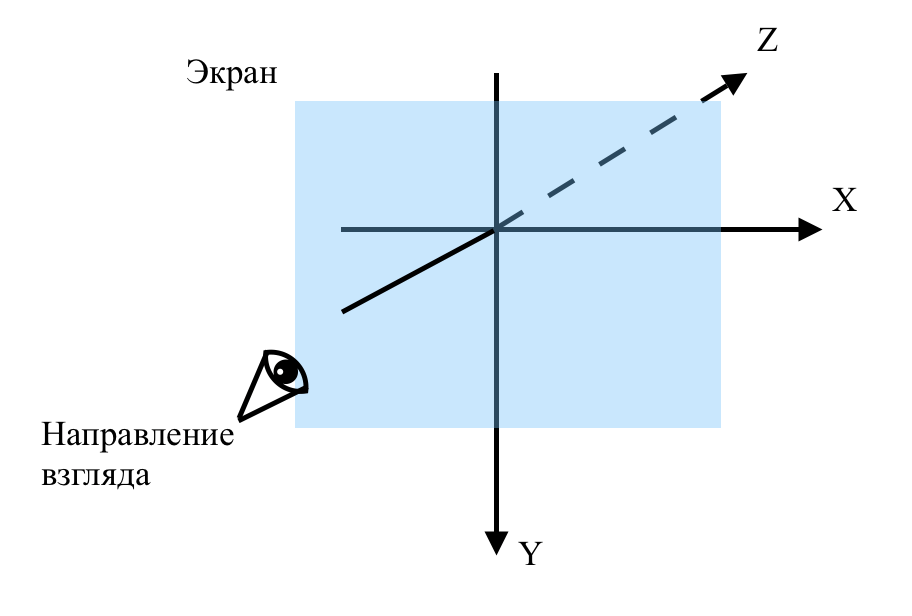
\includegraphics[scale=0.8]{coords}
	\caption{Экранная система координат с позицией камеры в начальный момент}
	\label{img:coords}
\end{figure}

Экран - прямоугольник, называется окном просмотра. В сущности, на холсте отображается всё то, что видим через окно просмотра.

Далее необходимо определить для каждого пикселя окна просмотра ($V$) какого же он цвета.

В реальном мире свет исходит из источника света (солнца, лампочки и т.д.), отражается от нескольких объектов и наконец достигает наших глаз. Необходимо трассировать лучи «в обратном порядке» -- следует начать с луча, находящегося на камере, проходящего через точку в окне просмотра и двигаясь, пока он не столкнётся с каким-нибудь объектом в сцене. Этот объект будет «виден» из камеры через эту точку окна просмотра. То есть в качестве первого приближения следует взять цвет этого объекта как «цвет света, прошедшего через эту точку».
Алгоритм представлен на рисунке \ref{img:raytrace}. 

\begin{figure}[H]
	\centering
	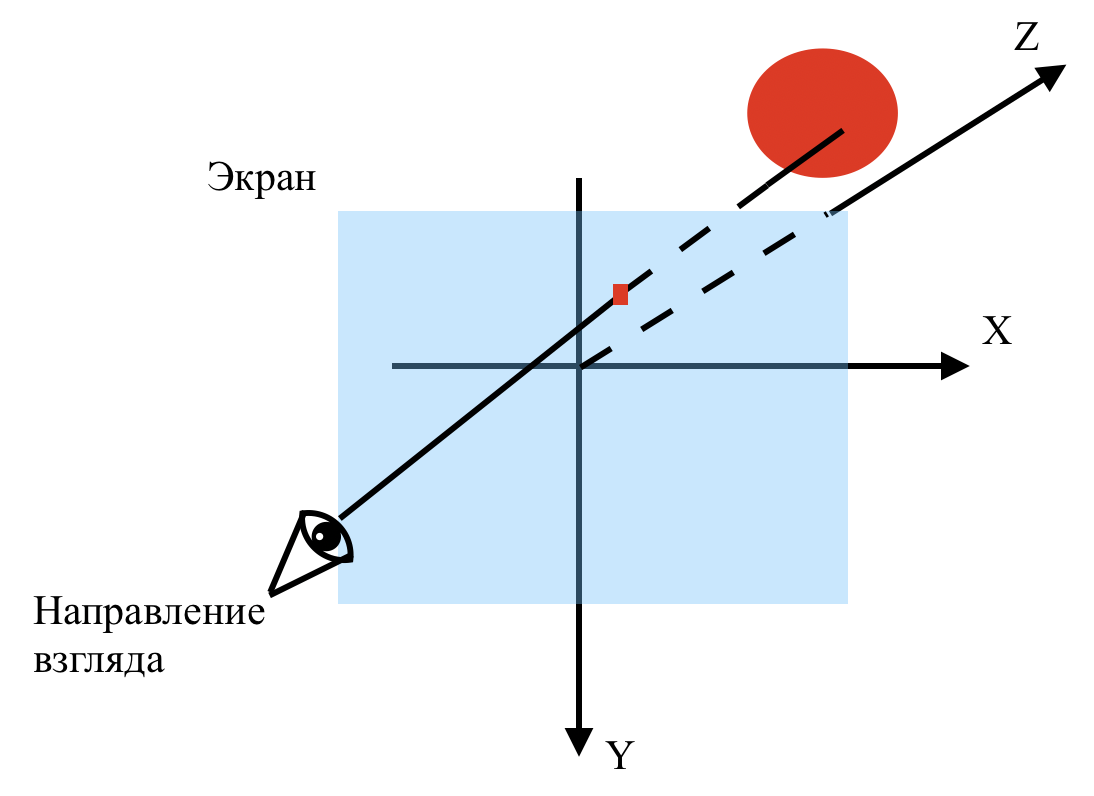
\includegraphics[scale=0.7]{raytrace}
	\caption{1 шаг алгоритма трассировки лучей}
	\label{img:raytrace}
\end{figure}

Наилучшим способом представления лучей для поставленной цели будет использование параметрического уравнения. Луч проходит через $O$, и его направление (из $O$ в $V$), поэтому любую точку $P$ луча можно представить как $P = O + t \cdot (V - O)$, где $t$ -- произвольное действительное число. 

Обозначим направление луча за $\vec D = \overrightarrow{(V - O) }$. Тогда уравнение примет вид: $P = O + t\vec D$. 

Следующим шагом необходимо рассмотреть объекты сцены, с которыми лучи сталкиваются. В сцене присутствует плоскость и сферы.

Для отыскания точки пересечения луча с произвольной поверхностью необходимо знать аналитические уравнения, определяющие оба эти объекта в трехмерном пространстве. Точка пересечения удовлетворяет всем уравнениям, так как принадлежит и лучу, и поверхности. Поэтому, сводя уравнения в систему и находя ее решения, мы получаем координаты этой точки. 

\textbf{Пересечение со сферой. }

Пусть из точки $O$ выпущен луч в направлении $\vec d$, как показано на рисунке \ref{img:sphera}. 

\begin{figure}[H]
	\centering
	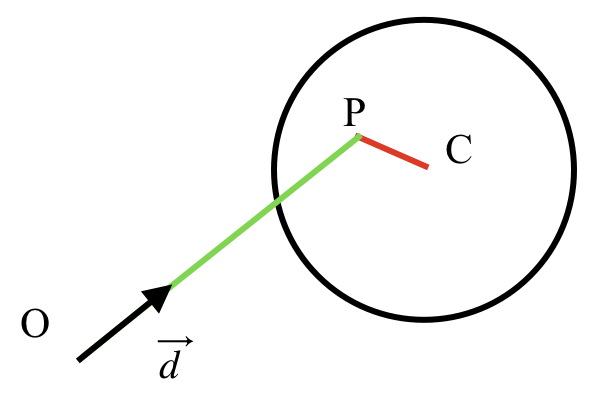
\includegraphics[scale=0.7]{sphera}
	\caption{Пересечение луча со сферой}
	\label{img:sphera}
\end{figure}

Точкой пересечения луча и сферы является $P$ -- решение системы  \ref{eq:sphera}. 

\begin{equation}
	\centering
	\begin{cases}
   		P = O + t\vec d\\
   		(P-C)^2 = r^2
 	\end{cases}
	\label{eq:sphera}
\end{equation}

$$(O + t\vec d - C) ^ 2 = r^2$$
$$\text{Обозначим }\vec s = C - A  \text{, тогда }$$
$$(t\vec d -\vec s)^2 = r^2$$
$$t^2 \vec d^2  - 2  t \cdot (\vec d, \vec s) + \vec s ^2 = r^2$$, где $(d,s)$ — скалярное произведение $\vec d $ и$ \vec s$, равное сумме попарных произведений их координат.

Получилось квадратное уравнение. 

$$D = (\vec d, \vec s)^2- \vec d^2 (\vec s ^2- r^2)$$

Если $D < 0$, то луч проходит мимо сферы, если же $D \le 0$, то уравнение имеет действительные корни:

$$t_{1,2}=\frac{(\vec d, \vec s) \pm sqrt(D) }{\vec d^2}$$

Наименьшее положительное значение $t$, если оно существует, дает ответ задачи. Если же положительного значения нет, то луч сферу не пересекает.

Если точка пересечения найдена, то нас будет интересовать также нормаль к поверхности в этой точке, так как эта нормаль определяет направление отраженного луча. Формула \ref{eq:normalsphere}. 

\begin{equation}
	\centering
   		\vec n = \frac{P - O}{|P-O|}
	\label{eq:normalsphere}
\end{equation}

\textbf{Пересечение с плоскостью. }

Плоскость задается общим уравнением: $(P, n) = r$, где $n$ -- вектор нормали с плоскости, имеющий единичную длину, а $r$ -- расстояние от начала координат до плоскости (с точностью до знака). См. рисунок \ref{img:plane}. 

\begin{figure}[H]
	\centering
	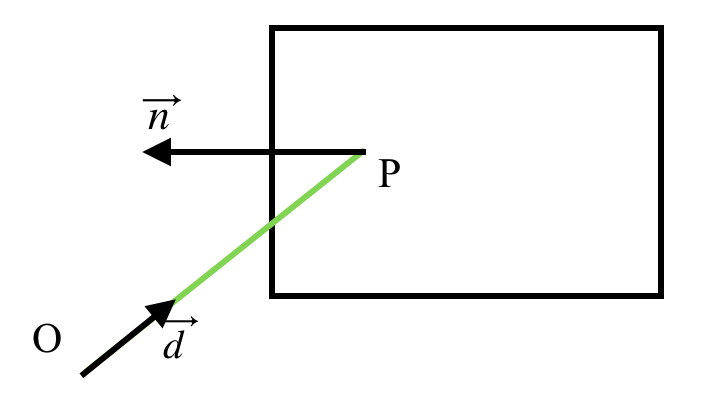
\includegraphics[scale=0.7]{plane}
	\caption{Пересечение луча с плоскостью}
	\label{img:plane}
\end{figure}

Точкой пересечения луча и плоскости является $P$ -- решение системы  \ref{eq:plane}. 

\begin{equation}
	\centering
	\begin{cases}
   		P = O + t\vec d\\
   		(P, \vec n) = r
 	\end{cases}
	\label{eq:plane}
\end{equation}

Тогда:

$$t = \frac{r - (O, \vec n)}{(\vec d, \vec n)}$$

Если $(d,n) = 0$, то луч параллелен плоскости, т.е. не пересекает ее. Если же $(d,n) \ne 0$, то вычисляем t. Тогда если его значение положительно, то луч пересекает плоскость.

\textbf{Источники освещения}

Свет должен откуда-то поступать. 

Точечный источник испускает свет из фиксированной точки в пространстве, называемой его позицией. Свет испускается равномерно во всех направлениях; именно поэтому его также называют всенаправленным освещением. Следовательно, точечный источник полностью характеризуется его позицией и яркостью.

Тогда $\vec l$ -- направление из точки $P$ в сцене к источнику освещения $Q$. Этот вектор, называемый световым вектором, просто равен  $\overrightarrow{Q-P}$. 

Для вычисления освещённости точки нам просто нужно вычислить количество света, вносимое каждым источником и сложить их, чтобы получить одно число, представляющее общее количество полученного точкой освещения. Затем необходимо вычислить новое значение цвета пикселя, используя цветовую модель HSV (англ. Hue, Saturation, Value — тон, насыщенность, значение). 

\textbf{Диффузное рассеяние}

Когда луч света падает на матовый объект, то из-за неровностей его поверхности, он отражает луч в сцену равномерно во всех направлениях, то есть получается «рассеянное» («диффузное») отражение.

С другой стороны, количество отражённого света зависит от угла между лучом света и поверхностью. Интуитивно это понятно -- энергия, переносимая лучом, в зависимости от угла должна распределиться по меньшей или большей поверхности, то есть энергия на единицу площади, отражённая в сцену, будет соответственно выше или ниже. 

Чтобы выразить это математически, используется вектор нормали. Вектор нормали, или просто «нормаль» — это вектор, перпендикулярный поверхности в какой-то точке. Также он является единичным вектором, то есть его длина равна 1. См. формулу \ref{eq:normalsphere} или уравнение плоскости. 

Итак, луч света с направлением $\vec l$ и яркостью $I$ падает на поверхность с нормалью $\vec n$. Какая часть $I$ отражается обратно на сцену. Схема диффузного отражения изображена на рисунке \ref{img:diffusion}. 

\begin{figure}[H]
	\centering
	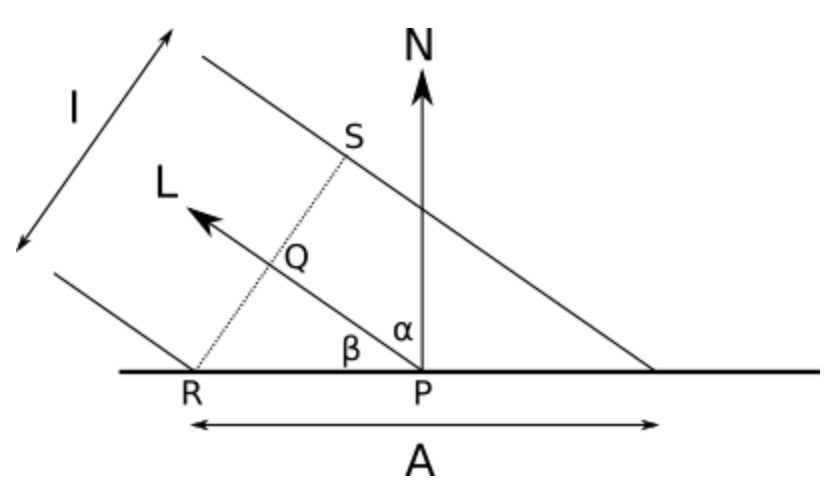
\includegraphics[scale=0.7]{diffusion}
	\caption{Диффузное отражение}
	\label{img:diffusion}
\end{figure}

Поскольку технически луч света не имеет ширины, поэтому считается, что всё происходит на бесконечно малом плоском участке поверхности. Даже если это поверхность сферы, то рассматриваемая область настолько бесконечно мала, что она почти плоская относительно размера сферы, так же как Земля выглядит плоской при малых масштабах.

Луч света с яркостью $I$ падает на поверхность в точке $P$ под углом  $\beta$. Нормаль в точке $P$ равна $\vec n$, а энергия, переносимая лучом, распределяется по A. Нам нужно вычислить $\frac{I}{A}$.

Будем считать $SR$ «шириной» луча. По определению, она перпендикулярна $\vec l$, который также является направлением $PQ$. Поэтому $PQ$ и $QR$ образуют прямой угол. 

Давайте рассмотрим треугольник $PQR$. 

$$QR = \frac{I}{2}$$
$$PR = \frac{A}{2}$$

Тогда

$$cos(\alpha) = \frac{QR}{PR} = \frac{I}{A}$$
 
$\alpha$ -- угол между $\vec n$ и $\vec l$. То есть

$$cos(\alpha) = \frac{(\vec n, \vec l)}{|\vec n||\vec L|}$$

\textbf{Тени}

Тени появляются там, где есть свет, но его лучи не могут достичь объекта, потому что на их пути есть другой объект.

Рассматривается луч, который проходит из точки до источника освещения. Пересекает ли этот луч другой объект? Если нет, то между точкой и источником ничего нет, то есть мы можем вычислить освещённость от этого источника и прибавить его к общей освещённости. Если пересекает, то мы игнорируем этот источник. См. рисунок \ref{img:shadows}. 

\begin{figure}[H]
	\centering
	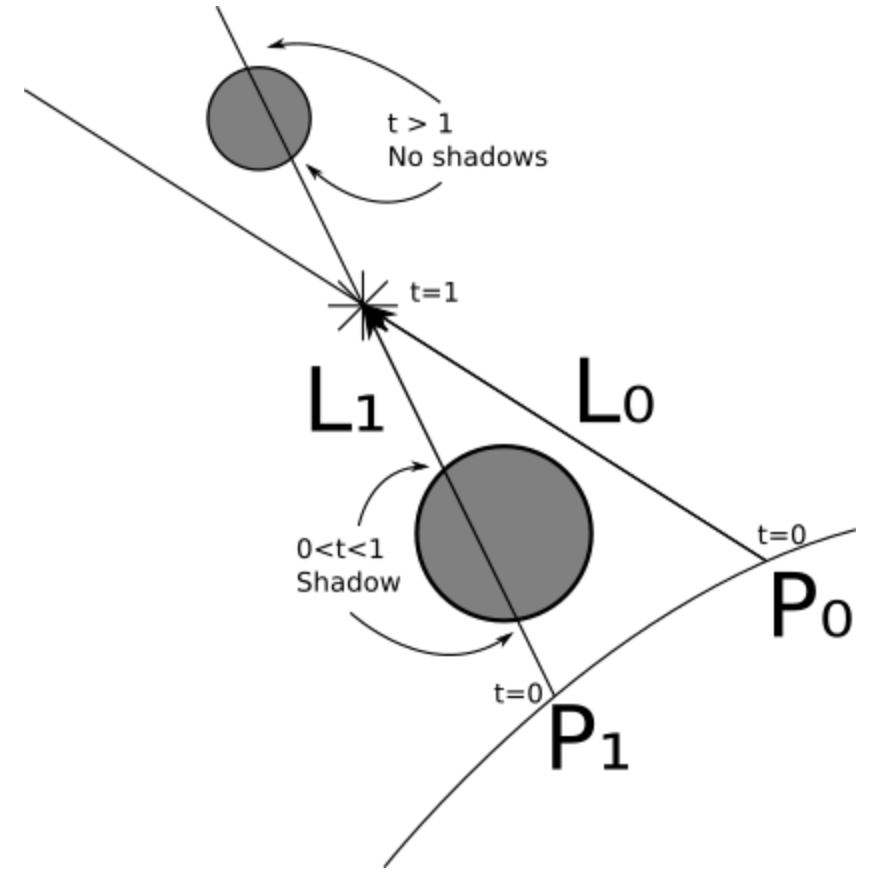
\includegraphics[scale=0.7]{shadows}
	\caption{Тени}
	\label{img:shadows}
\end{figure}

Существует один пограничный случай, который нам нужно рассмотреть. Если искать пересечения, начиная с $t=0$ то мы, вероятнее всего, найдём саму $P$, другими словами, каждый объект будет отбрасывать тени на самого себя. 

Простейший способ справиться с этим — использовать в качестве нижней границы значений $t$ вместо 0 использовать малое значение $\epsilon$. 

\subsection{\textbf{Моделирование взрыва}}

\hfill

Взрыв частиц состоит из взаимодействия между каждой парой частиц. Приведенное ниже столкновение является описанием события 3D-столкновения и обеспечивает сохранение импульса и энергии.

Рассматриваются 2 частицы $m1,~ m2$ с радиусами $r1,~r2$, центры которых находятся в точках с координатами $(x1,y1,z1),~(x2,y2,z2)$ и двигаются со скоростями $(vx1,vy1,vz1),~(vx2,vy2,vz2)$. 

\textbf{Алгоритм. }
\begin{enumerate}
	\item Вычислить относительное расстояние и относительную скорость. 
	
	\item Если расстояние между шарами больше суммы радиусов или если относительная скорость = 0 (частицы не взаимодействуют) $\to$ выход из подпрограммы. 
	
	\item Для моделирования необходимо перейти в систему координат, одна из осей которой направлена вдоль вектора скорости 2 шара (он покоится), а начало координат совпадает с центром первой частицы. См. рисунок  \ref{img:coords_explosion}. 
	
	Для этого необходимо сдвинуть систему координат так, чтобы шар 1 находился в начале координат, а затем изменить скорость 1 шара на относительную (так как 2 шар покоится в новой системе отсчета). Для того чтобы ось $Z$ была направлена вдоль вектора $v_2$, необходимо сделать два поворота: первый -- на угол $\varphi$ вокруг оси Z, второй -- на угол $\theta$ вокруг оси Y.
	
	\begin{figure}[H]
		\centering
		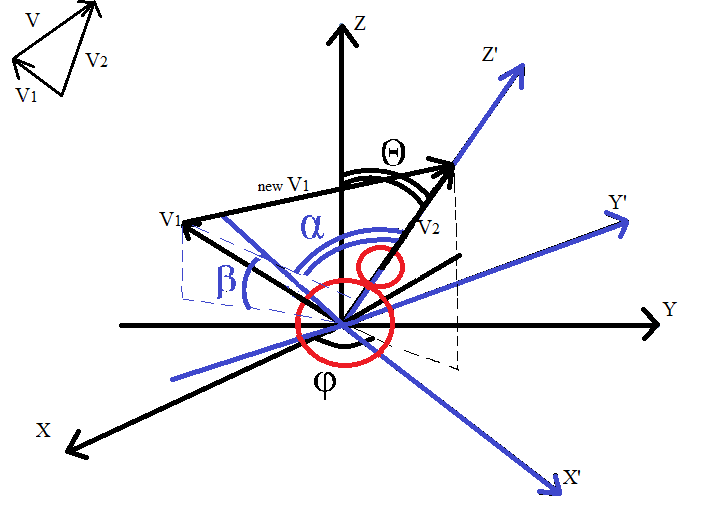
\includegraphics[scale=0.6]{coords_explosion}
		\caption{}
		\label{img:coords_explosion}
	\end{figure}
	
	Матрица первого поворота
	
	\begin{equation}
		\begin{pmatrix}
			cos(\varphi)& sin(\varphi) & 0\\
			-sin(\varphi)& cos(\varphi) & 0\\
			0&0&1
		\end{pmatrix}
		\label{eq:matr_varphi}
	\end{equation}
	
	Матрица второго поворота
	
	\begin{equation}
		\begin{pmatrix}
			cos(\theta)& 0 & -sin(\theta)\\
			0& 1 & 0\\
			sin(\theta)&0&cos(\theta)
		\end{pmatrix}
		\label{eq:matr_theta}
	\end{equation}
	
	Пересчет координат вектора при переходе от системы $XYZ$ к системе $X',Y',Z'$ дается произведением матриц \ref{eq:matr_varphi}, \ref{eq:matr_theta}. 
	
	\begin{equation}
		\begin{pmatrix}
			cos(\theta)cos(\varphi)& cos(\theta)sin(\varphi) & -sin(\theta)\\
			-sin(\varphi)& cos(\varphi) & 0\\
			sin(\theta)cos(\varphi)&sin(\theta)sin(\varphi)&cos(\theta)
		\end{pmatrix}
		\label{eq:matr_rotate}
	\end{equation}
	
	Обратный переход от системы $X',Y',Z'$ к системе $XYZ$ производится с помощью транспонированной матрицы. 
	
	\begin{equation}
		\begin{pmatrix}
			cos(\theta)cos(\varphi)& -sin(\varphi) & sin(\theta)cos(\varphi)\\
			cos(\theta)sin(\varphi)& cos(\varphi) & sin(\theta)sin(\varphi)\\
			-sin(\theta)&0&cos(\theta)
		\end{pmatrix}
		\label{eq:matr_transpose}
	\end{equation}
	
	\item Проверить сталкиваются ли шары (пересечение векторов скоростей) $\to$ если нет, выход из-под программы. 
	\item Нахождение новых скоростей, решением системы уравнений \ref{eq:system}.  
	
	\begin{equation}
		\begin{matrix}
			m_1 v_{1,x} = m_1 v_{1,x}' + m_2 v_{2,z}' tg(\alpha)cos(\beta)\\
			m_1 v_{1,y} = m_1 v_{1,y}' + m_2 v_{2,z}'tg(\alpha)sin(\beta)\\
			m_1 v_{1,z} = m_1 v_{1,z}' + m_2 v_{2,z}'\\
			\frac{m_1(v_{x,1}^2+v_{y,1}^2+v_{z,1}^2) }{2} =  \frac{m1(v_{x,1}'^2+v_{y,1}'^2+v_{z,1}'^2)}{2} + \frac{m2v_{z,2}'^2(1+tg^2(\alpha))}{2} 
		\end{matrix}
		\label{eq:system}
	\end{equation}

	\item Обновить скорости и повернуть векторы скорости назад и добавить начальный вектор скорости шара 2, чтобы получить исходную систему координат. 
	
\end{enumerate}

\section{\textbf{Разработка и обоснование используемых типов и структур данных }}

В данной работе происходит взаимодействие с моделью, структура которой представлена на рисунке \ref{img:model}. Состоит из вектора частиц (система частиц, в которой каждая частица обладает определенными параметрами), земля -- плоскость, на которой происходит взаимодействие частиц и частица, рассматриваемая отдельно, в начальный момент имеющая скорость. 

\begin{figure}[H]
	\centering
	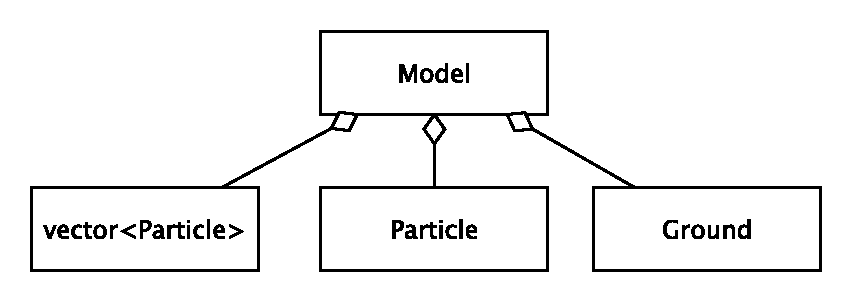
\includegraphics[scale=0.7]{model}
	\caption{Структура модели}
	\label{img:model}
\end{figure}

Камера в данной работе содержит структуру матрицу, для удобства взаимодействия. В ней реализованы методы, умножения матрицы на матрицу, вектора на матрицу для работы с преобразования координат. 

\begin{figure}[H]
	\centering
	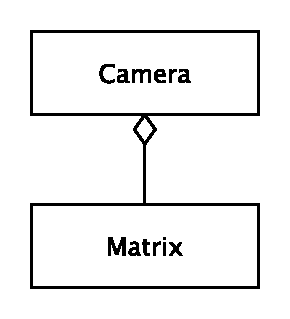
\includegraphics[scale=0.7]{camera}
	\caption{Структура камеры}
	\label{img:camera}
\end{figure}

\section{\textbf{Разработка структуры программного комплекса}}
\hfill

Алгоритм работы программы. 
\begin{enumerate}
	\item[1. ] Загрузка модели из txt файла.
	\item[2. ] Установка первоначальных параметров для модели сцены и камеры. 
	\item[3. ] Вычисление координат и положения объекта (для различных этапов взрыва). 
	\item[4. ] Преобразование координат (повороты моделей, масштабирование и перенос) относительно камеры.
	\item[5. ] Генерация и отображение модели. 
	\item[6. ] Считывание новых параметров. 
	\item[7. ] Возвращение к п.3. 
\end{enumerate}

\section{\textbf{Вывод}}

\hfill

Необходимо реализовать алгоритмы трассировки лучей для удаления невидимых поверхностей и работы с освещением (диффузное отражение и тени). Далее необходимо разработать алгоритм визуализации взрыва с опорой на физические законы, такие как закон сохранения энергии и закон сохранения импульса. 

Необходимо также разработать взаимодействие с камерой и объектом (перемещение, масштабирование, поворот). 
